\documentclass[10pt,landscape]{article}
\usepackage[letterpaper,landscape,margin=0.42in]{geometry}
\usepackage{newpxtext,newpxmath}
\usepackage{microtype}
\usepackage{xcolor,pagecolor}
\usepackage{amsmath}
\usepackage{tikz}
\usetikzlibrary{arrows.meta,positioning}
\usepackage[most]{tcolorbox}
\definecolor{Paper}{HTML}{FFFDF8}
\definecolor{Navy}{HTML}{0B1F33}
\definecolor{Blue}{HTML}{2F63D6}
\definecolor{Teal}{HTML}{17A99A}
\definecolor{Gold}{HTML}{D8A62E}
\definecolor{SoftGold}{HTML}{FFF5D8}
\definecolor{SoftBlue}{HTML}{EDF4FF}
\definecolor{SoftTeal}{HTML}{EAF9F6}
\definecolor{Line}{HTML}{D9DEE8}
\pagecolor{Paper}
\color{Navy}
\pagestyle{empty}
\setlength{\parindent}{0pt}
\setlength{\parskip}{2pt}
\tcbset{enhanced, boxrule=0.45pt, arc=2mm, left=2mm, right=2mm, top=1.5mm, bottom=1.5mm}
\newtcolorbox{card}[1]{colback=white,colframe=Line,borderline west={2pt}{0pt}{Gold},title=\sffamily\bfseries #1,coltitle=Navy,colbacktitle=SoftBlue,detach title,before upper={\tcbtitle\par\vspace{1mm}\scriptsize}}
\newtcolorbox{hero}{colback=SoftGold,colframe=Gold,boxrule=0.55pt,arc=2mm,left=2mm,right=2mm,top=1.3mm,bottom=1.3mm,fontupper=\bfseries\sffamily\color{Navy}}
\begin{document}
{\sffamily\bfseries\Large GoalOS Mission OS}\hfill{\sffamily\bfseries\color{Gold} The Proof OS for Autonomous AI Work}\par
{\sffamily Set the objective. GoalOS runs until proof is done.}\vspace{2mm}
\begin{hero}AI creates output. GoalOS creates proof. The deliverable is not a document; it is a governed decision state.\end{hero}
\vspace{2mm}
\begin{minipage}[t]{0.31\linewidth}
\begin{card}{Publication law}
Website publication is governed work:\par
\vspace{1mm}
Content source $\rightarrow$ Generator $\rightarrow$ QA $\rightarrow$ PR $\rightarrow$ Human review $\rightarrow$ Live site $\rightarrow$ Chronicle.
\end{card}
\begin{card}{Mission loop}
Objective $\rightarrow$ Mission Contract $\rightarrow$ Autonomous Work $\rightarrow$ Verification $\rightarrow$ Evidence Docket $\rightarrow$ Decision State $\rightarrow$ Action Graph $\rightarrow$ Chronicle.
\end{card}
\begin{card}{Canonical doctrine}
A model can answer. An agent can act. An institution must prove. No proof, no settlement. No eval, no propagation. No rollback, no release.
\end{card}
\end{minipage}\hfill
\begin{minipage}[t]{0.33\linewidth}
\begin{card}{Mission value}
\[
\mathrm{MissionValue}=\frac{DI\cdot PI\cdot A\cdot R}{C+Risk+L+PD}
\]
\vspace{-2mm}
\begin{tabular}{ll}
$DI$ & Decision impact \\
$PI$ & Proof integrity \\
$A$ & Actionability \\
$R$ & Reuse \\
$PD$ & Proof debt
\end{tabular}
\end{card}
\begin{card}{Proof-to-action law}
\[
AIWork=Output\cdot Proof\cdot Validation\cdot Actionability\cdot Reuse
\]
If $Proof=0$, trusted institutional work is zero.
\end{card}
\begin{card}{Publish readiness}
\[
PublishReady=C_v\land B_p\land Q_p\land C_b\land H_r
\]
Content valid, build pass, QA pass, claim boundary pass, human review.
\end{card}
\end{minipage}\hfill
\begin{minipage}[t]{0.31\linewidth}
\begin{card}{Governed decision state}
Mission Contract; Claims Matrix; Source Provenance; Contradiction Register; Evidence Docket; Verifier Report; Risk Ledger; Executive Brief; Action Graph; Chronicle; Capability Package.
\end{card}
\begin{card}{AGIALPHA boundary}
$AGIALPHA$ is proof-settlement fuel: budget, escrow, stake, validation, settlement, reputation, and treasury routing. It is not equity, yield, profit share, ownership, or guaranteed return.
\end{card}
\begin{card}{Claim boundary}
No achieved AGI/ASI claim. No guaranteed ROI claim. No production-security or external-audit claim without evidence. No Mainnet deployment claim without chain evidence.
\end{card}
\end{minipage}
\vspace{2mm}
\begin{center}
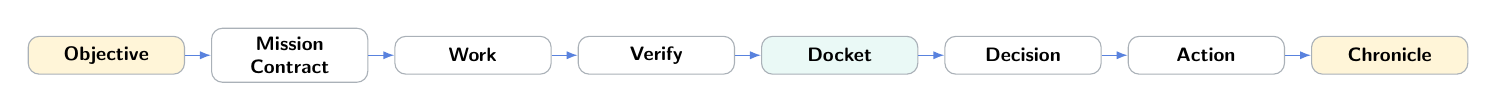
\begin{tikzpicture}[node distance=0.33cm, every node/.style={font=\scriptsize\sffamily\bfseries}, box/.style={rounded corners=1.4mm, draw=Navy!35, fill=white, minimum height=0.48cm, align=center, text width=1.75cm}, arrow/.style={-{Latex[length=1.4mm]}, line width=0.5pt, color=Blue!80}]
\node[box,fill=SoftGold] (o) {Objective};
\node[box,right=of o] (mc) {Mission Contract};
\node[box,right=of mc] (aw) {Work};
\node[box,right=of aw] (vf) {Verify};
\node[box,right=of vf,fill=SoftTeal] (ed) {Docket};
\node[box,right=of ed] (ds) {Decision};
\node[box,right=of ds] (ag) {Action};
\node[box,right=of ag,fill=SoftGold] (ch) {Chronicle};
\foreach \x/\y in {o/mc,mc/aw,aw/vf,vf/ed,ed/ds,ds/ag,ag/ch}{\draw[arrow] (\x)--(\y);}
\end{tikzpicture}
\end{center}
\begin{hero}The website is generated from proof-aligned source, checked by automation, reviewed by a human, and then published.\end{hero}
\end{document}
